\section{Anexos}

\textbf{Anexo 1. Esquema del problema}

\begin{figure}[H]
\centering
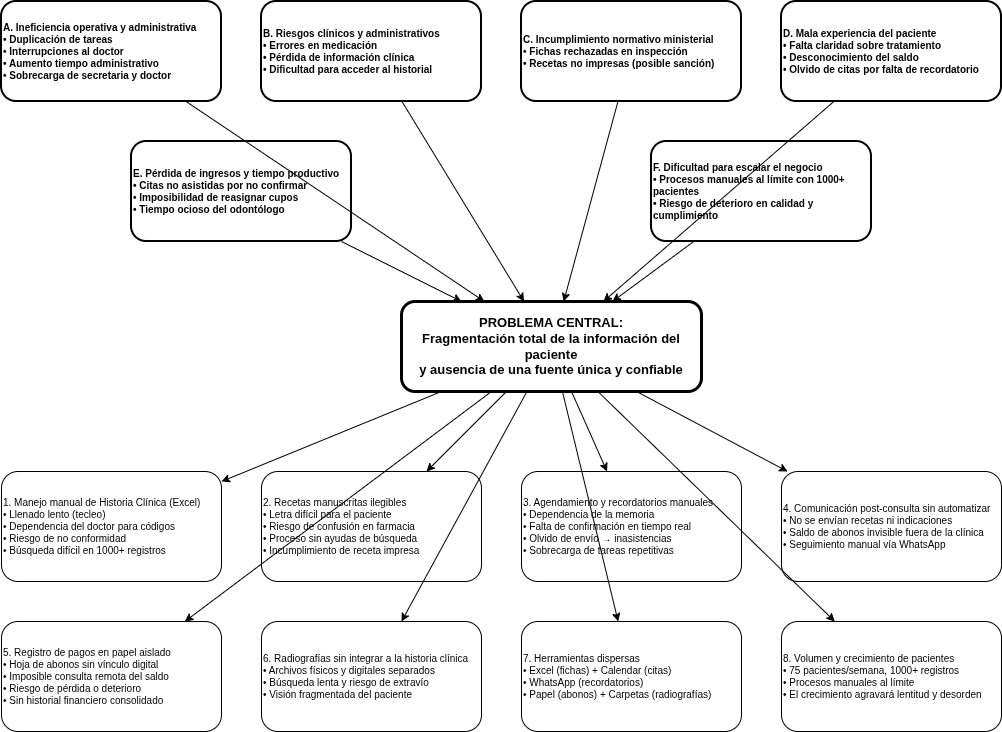
\includegraphics[width=\linewidth]{img/problem-scheme_bn.png}
\caption{Esquema del problema.}
\label{fig:esquema-problema}
\end{figure}

\newpage
\textbf{Anexo 2. Instrumento N.\textsuperscript{o}~1:
Entrevista estructurada}

\begin{table}[H]
\centering
\renewcommand{\arraystretch}{1.3}
\begin{tabular}{|p{3.5cm}|p{10.2cm}|}
\hline
\multicolumn{2}{|l|}{\textbf{Datos de identificación}} \\ \hline
Fecha:               & \\ \hline
Hora de inicio:      & \\ \hline
Hora de finalización:& \\ \hline
Entrevistador:       & \\ \hline
Rol del entrevistado:&
  $\square$~Odontólogo general \quad
  $\square$~Odontólogo especialista \quad
  $\square$~Secretaria \\ \hline
\end{tabular}
\end{table}

\noindent\textbf{Instrucciones.} La entrevista es individual y
confidencial. No existen respuestas correctas o incorrectas; el
objetivo es conocer con la mayor precisión posible el flujo de
trabajo actual del consultorio. Se solicita responder con
sinceridad y con el nivel de detalle que cada pregunta requiera.
La duración estimada es de 25 a 35 minutos.

\bigskip
\noindent\textbf{Bloque~I — Flujo actual de trabajo diario por rol}

\begin{enumerate}
\item ¿Cuáles son las tareas que usted realiza desde que llega
al consultorio hasta que atiende al primer paciente del día?
Descríbalas en orden.

\vspace{2.8cm}

\item ¿Cómo se registran los datos de un paciente nuevo?
¿Qué herramientas o formatos utiliza en ese proceso?

\vspace{2.8cm}

\item ¿De qué manera accede a la historia clínica de un paciente
durante la consulta? ¿Dónde se almacena y quién puede
consultarla?

\vspace{2.8cm}

\item ¿Cómo se registra la información generada durante la
consulta (diagnóstico, tratamiento realizado, receta)?
¿Lo hace usted mismo o interviene otra persona?

\vspace{2.8cm}

\item ¿Cómo se gestiona el cobro al paciente y la emisión del
comprobante? ¿Qué pasos sigue ese proceso desde que termina
la consulta?

\vspace{2.8cm}
\end{enumerate}

\bigskip
\noindent\textbf{Bloque~II — Problemas, retrasos e interrupciones}

\begin{enumerate}
\setcounter{enumi}{5}
\item ¿En qué momentos del día siente que el trabajo se retrasa
o se complica más? ¿A qué lo atribuye?

\vspace{2.8cm}

\item ¿Ha tenido situaciones en que no encontraba la historia
clínica de un paciente o la información estaba incompleta?
¿Cómo resolvió ese problema?

\vspace{2.8cm}

\item ¿Existen tareas que tenga que repetir o ingresar más de
una vez en distintos documentos o herramientas? Descríbalas.

\vspace{2.8cm}

\item ¿Ha ocurrido alguna vez que se perdiera información
importante de un paciente? ¿Cuál fue la consecuencia?

\vspace{2.8cm}

\item ¿Qué parte del proceso administrativo considera que consume
más tiempo innecesario durante la jornada de trabajo?

\vspace{2.8cm}
\end{enumerate}

\bigskip
\noindent\textbf{Bloque~III — Cumplimiento de normas y registro
clínico}

\begin{enumerate}
\setcounter{enumi}{10}
\item ¿Conoce los requisitos del Ministerio de Salud Pública
sobre la historia clínica odontológica (Formulario~033 y
Acuerdo Ministerial 5216-A)? ¿Los aplica actualmente?

\vspace{2.8cm}

\item ¿Todos los campos obligatorios del Formulario~033 se
completan de manera habitual? Si no es así, ¿cuáles se omiten
con mayor frecuencia y por qué?

\vspace{2.8cm}

\item ¿Cómo se archivan las historias clínicas actualmente?
¿Existe algún procedimiento para su custodia y acceso?

\vspace{2.8cm}

\item ¿Se registran las recetas emitidas de forma que puedan
recuperarse posteriormente si el paciente regresa?

\vspace{2.8cm}

\item ¿Considera que el sistema actual de registro cumple con
las exigencias legales vigentes? Explique su respuesta.

\vspace{2.8cm}
\end{enumerate}

\bigskip
\noindent\textbf{Bloque~IV — Funciones esperadas del nuevo sistema}

\begin{enumerate}
\setcounter{enumi}{15}
\item ¿Qué tareas del proceso administrativo le gustaría que el
nuevo sistema realizara de forma automática o más rápida?

\vspace{2.8cm}

\item ¿Qué información considera indispensable tener disponible
de manera inmediata durante la atención al paciente?

\vspace{2.8cm}

\item ¿Existe alguna función que, en su opinión, no debería
incluirse o que podría generar complicaciones al personal?

\vspace{2.8cm}

\item ¿Cómo prefiere que el sistema le presente la información:
en pantallas simples con pocos campos a la vez o con toda la
información del paciente en una sola vista?

\vspace{2.8cm}

\item ¿Hay algún aspecto del trabajo diario que no haya sido
abordado en esta entrevista y que considere relevante para
el diseño del sistema?

\vspace{2.8cm}
\end{enumerate}

\noindent\rule{\linewidth}{0.4pt}
\noindent\textit{Observaciones adicionales del entrevistador:}
\vspace{3cm}

% ============================================================
% ANEXO 2 — INSTRUMENTO N.º 2: FICHA DE OBSERVACIÓN
% ============================================================

\newpage
\textbf{Anexo 3. Instrumento N.\textsuperscript{o}~2:
Ficha de observación de procesos}

\begin{table}[H]
\centering
\renewcommand{\arraystretch}{1.3}
\begin{tabular}{|p{3.5cm}|p{10.2cm}|}
\hline
\multicolumn{2}{|l|}{\textbf{Datos de identificación}} \\ \hline
Fecha:               & \\ \hline
Hora de inicio:      & \\ \hline
Hora de finalización:& \\ \hline
Observador:          & \\ \hline
Actor observado:     &
  $\square$~Odontólogo general \quad
  $\square$~Odontólogo especialista \quad
  $\square$~Secretaria \\ \hline
\end{tabular}
\end{table}

\noindent\textbf{Instrucciones.} El observador no intervendrá en
ninguna actividad del consultorio. Se registrará todo lo observado
de forma objetiva, evitando interpretaciones. La jornada de
observación tiene una duración de aproximadamente seis horas,
equivalente a la jornada laboral habitual.

\bigskip
\noindent\textbf{Sección~A — Inventario de herramientas y archivos
de información utilizados}

\begin{table}[H]
\centering
\renewcommand{\arraystretch}{1.5}
\begin{tabular}{|p{0.5cm}|p{4.0cm}|p{3.8cm}|p{5.3cm}|}
\hline
\textbf{N.\textsuperscript{o}} &
\textbf{Herramienta / archivo} &
\textbf{Tipo}
  (\textit{físico / digital}) &
\textbf{Uso observado} \\ \hline
1  & & & \\ \hline
2  & & & \\ \hline
3  & & & \\ \hline
4  & & & \\ \hline
5  & & & \\ \hline
6  & & & \\ \hline
7  & & & \\ \hline
8  & & & \\ \hline
\end{tabular}
\end{table}

\noindent\textit{Notas abiertas sobre herramientas:}
\vspace{2.5cm}

\bigskip
\noindent\textbf{Sección~B — Secuencia de tareas por etapa del
ciclo de atención}

\begin{table}[H]
\centering
\renewcommand{\arraystretch}{1.8}
\setlength{\tabcolsep}{3pt}
\begin{tabular}{|p{0.5cm}|p{2.6cm}|p{1.8cm}|p{2.6cm}|p{2.0cm}|p{3.4cm}|}
\hline
\textbf{N.\textsuperscript{o}} &
\textbf{Tarea observada} &
\textbf{Encargado} &
\textbf{Herramienta usada} &
\textbf{T.\ estimado (min)} &
\textbf{Interrupciones / incidencias} \\ \hline
\multicolumn{6}{|l|}{\textit{Antes de la consulta}} \\ \hline
1 & & & & & \\ \hline
2 & & & & & \\ \hline
3 & & & & & \\ \hline
4 & & & & & \\ \hline
\multicolumn{6}{|l|}{\textit{Durante la consulta}} \\ \hline
5 & & & & & \\ \hline
6 & & & & & \\ \hline
7 & & & & & \\ \hline
8 & & & & & \\ \hline
\multicolumn{6}{|l|}{\textit{Después de la consulta}} \\ \hline
9  & & & & & \\ \hline
10 & & & & & \\ \hline
11 & & & & & \\ \hline
12 & & & & & \\ \hline
\end{tabular}
\end{table}

\bigskip
\noindent\textbf{Sección~C — Información aislada, tareas manuales
redundantes y tiempos de espera}

\begin{table}[H]
\centering
\renewcommand{\arraystretch}{1.5}
\begin{tabular}{|p{0.5cm}|p{4.8cm}|p{3.2cm}|p{4.8cm}|}
\hline
\textbf{N.\textsuperscript{o}} &
\textbf{Problema identificado} &
\textbf{Tipo}
  (\textit{info.\ aislada /}
  \textit{tarea redundante /}
  \textit{espera}) &
\textbf{Descripción detallada} \\ \hline
1 & & & \\ \hline
2 & & & \\ \hline
3 & & & \\ \hline
4 & & & \\ \hline
5 & & & \\ \hline
6 & & & \\ \hline
\end{tabular}
\end{table}

\noindent\rule{\linewidth}{0.4pt}
\noindent\textit{Observaciones generales del observador:}
\vspace{3cm}

% ============================================================
% ANEXO 3 — INSTRUMENTO N.º 3: FICHA DE REGISTRO DE TIEMPOS
% ============================================================

\newpage
\textbf{Anexo 4. Instrumento N.\textsuperscript{o}~3:
Ficha de registro del tiempo del ciclo administrativo}

\begin{table}[H]
\centering
\renewcommand{\arraystretch}{1.3}
\begin{tabular}{|p{3.5cm}|p{10.2cm}|}
\hline
\multicolumn{2}{|l|}{\textbf{Sección~A — Datos de identificación
del ciclo}} \\ \hline
N.\textsuperscript{o} de control: & \\ \hline
Fecha:                            & \\ \hline
Observador:                       & \\ \hline
Tipo de paciente:                 &
  $\square$~Paciente nuevo \quad
  $\square$~Paciente recurrente \\ \hline
Fase de medición:                 &
  $\square$~Pre-implementación (julio--agosto~2026) \quad
  $\square$~Post-implementación (noviembre~2026) \\ \hline
\end{tabular}
\end{table}

\noindent\textbf{Instrucciones.} El observador cronometrará
de forma continua cada subproceso, registrando la hora exacta
de inicio y fin sin interrumpir el flujo de atención. El ciclo
inicia cuando el paciente es registrado en recepción y concluye
cuando se emite el comprobante de pago. Anotar cualquier
interrupción observable en la columna correspondiente.

\bigskip
\noindent\textbf{Sección~B — Registro detallado por subproceso}

\begin{table}[H]
\centering
\renewcommand{\arraystretch}{1.9}
\setlength{\tabcolsep}{3pt}
\begin{tabular}{|p{0.5cm}|p{3.8cm}|p{1.8cm}|p{1.8cm}|p{1.8cm}|p{1.5cm}|p{2.0cm}|}
\hline
\textbf{N.\textsuperscript{o}} &
\textbf{Subproceso} &
\textbf{Encargado} &
\textbf{Hora inicio} &
\textbf{Hora fin} &
\textbf{Duración (min)} &
\textbf{Interrupciones} \\ \hline
1 & Registro de datos del paciente       & & & & & \\ \hline
2 & Búsqueda o apertura de historia
    clínica                              & & & & & \\ \hline
3 & Ingreso de datos de la consulta      & & & & & \\ \hline
4 & Generación de la receta              & & & & & \\ \hline
5 & Registro del pago                    & & & & & \\ \hline
6 & Emisión del comprobante              & & & & & \\ \hline
\end{tabular}
\end{table}

\bigskip
\noindent\textbf{Sección~C — Totales del ciclo de atención}

\begin{table}[H]
\centering
\renewcommand{\arraystretch}{1.5}
\begin{tabular}{|p{6.5cm}|p{7.2cm}|}
\hline
\textbf{Campo} & \textbf{Valor registrado} \\ \hline
Hora de inicio del ciclo           & \\ \hline
Hora de finalización del ciclo     & \\ \hline
\textbf{Tiempo total del ciclo (min)} & \\ \hline
Número total de interrupciones     & \\ \hline
Observaciones relevantes           &
  \vspace{1.8cm} \\ \hline
\end{tabular}
\end{table}

\noindent\rule{\linewidth}{0.4pt}
\noindent\textit{Verificado por:}
\hfill
\textit{Firma: \underline{\hspace{5cm}}}
\vspace{0.5cm}


\textbf{Anexo 5. Esquema metodológico}

\begin{figure}[H]
\centering
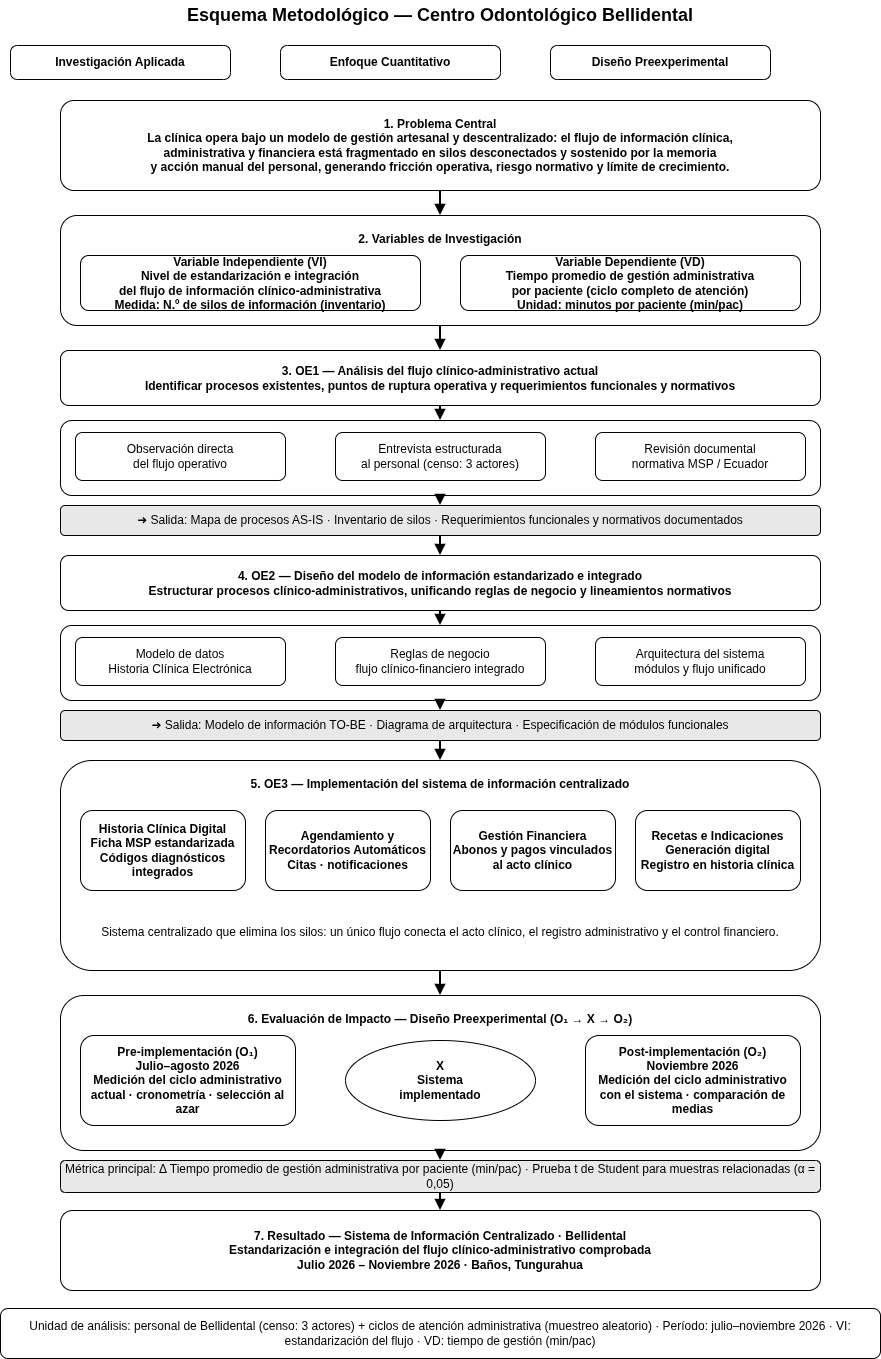
\includegraphics[width=\linewidth,
                 height=\dimexpr\textheight-2\baselineskip\relax,
                 keepaspectratio]{img/methodologic-scheme_bn}
\caption{Esquema metodológico.}
\label{fig:esquema-metodologico}
\end{figure}